\section{External Native Fault-Benchmark Methods}
\label{sec:limbo}

The complete schedule, execution sources, native implementation, wheel and runtime identities for the separately declared follow-up were published before its generation at protocol commit \texttt{\seqsplit{8b25d4c7769c5c593333c9d3eeeceb8ae001dba4}}. The protocol SHA-256 is \texttt{\seqsplit{6d34556a03e9d738d11367a40d4812cb93168c82d3ae775ef76f1a4c48679541}}. All 96 planned follow-up dispositions are retained, including errors and unavailable grades. Source, model and resource bindings are part of the accompanying audit-linked artifact. The original cohort at protocol commit \texttt{\seqsplit{267cd1a3e846c46c009f20accbf302746e064875}} was interrupted after 6/96 native grades became available. Its original final collector seal and process terminal are unavailable. A separately dated postcollection preservation archive binds copied original bytes; replay reconstructs only available sealed child returns. The remaining dispositions stay unknown, including the interrupted child and every unstarted slot. No original exit status or interruption cause is invented. Both 96-slot cohorts remain in the paper and artifact. The host migration required explicit runtime-path repairs, a new private runtime binding and a change from Ollama 0.40.8 to 0.40.10. The follow-up was declared after access to the partial original data. It reuses the same weights, frozen scientific sources, task indices, fault assignments, arm order, control settings, limits and analysis. It is a distinct runtime condition, not a resume, successful-slot replacement or independently sampled replication. Its within-world contrasts are primary; cross-cohort outcomes and costs are descriptive and never pooled. The two planned cohorts still contain only 12 unique base instances.

\subsection{Benchmark, selection, and matched conditions}

The external environment is the author-maintained LIMBO sandbox
\cite{limbo,limbosource}, pinned to commit
\texttt{\seqsplit{2db09fba22a0572a70639162a808906409f612a8}}. This source pin
differs from its \texttt{v1.0} tag
(\texttt{\seqsplit{83c59e31f8477a5fb6f186dfcc9f3d10fa336b8a}}); our executions
are not a reproduction of the preprint's released episode corpus. Native task
construction, service implementation, fault injection, policy prompts, tool
schemas, final settlement and grading remain unchanged. We use the minimal
native agent loop through a scoped policy-factory extension, rather than the
stock parallel runner and its retry/resume behavior. All services are simulated;
no production service write or real human intervention is involved.

The frozen schedule selected one parameterized base instance from each of
the 12 external templates across billing, data, deploy, mail, social and
tickets. Instance indices are hash-selected from the declared seed and index
salt, excluding development indices. A trusted extractor releases only
template/domain identifiers, focal-write names and public affordances for
selection; task instructions, targets, setup values and grader outcomes do not
enter the selection rule. Each base instance has a clean condition and one
compatible fault condition. Metadata-based balancing and hash tie-breaking
cover pre-dispatch timeout, post-commit timeout, late commit, heavy-tailed late
commit, partial-batch timeout and duplicate delivery; the batch-capable template
is reserved for the partial-batch condition. This is finite purposeful coverage,
not a random task sample or an exhaustive fault cross-product.

Four arms defined 24 task/fault conditions and 96 planned execution slots on
12 base instances. Rotating arm order balanced execution positions. Arms share
the native world within a condition, public capabilities, neutral tool
documentation, default instruction and resource limits. Clean and fault
conditions share base task parameters, but the native world RNG seed depends
on fault mode; they are not identical random worlds. The primary contrasts are
between arms within each world.

\begin{table}[t]
\caption{Frozen native comparison. The SDK arm preserves the supplied
strong guard's control law; it is a receipt-integration comparison.}
\label{tab:limbo-arms}
\centering\small
\setlength{\tabcolsep}{3pt}
\begin{tabular}{p{0.25\columnwidth}p{0.65\columnwidth}}
\toprule
Arm & Execution rule \\
\midrule
\texttt{vanilla} & Unchanged native direct tool dispatch. \\
\texttt{sdk\_retry3} & Unchanged native transparent retry rule: up to three
automatic retries after an initial retryable failure, with native backoff. \\
\texttt{guard} & Unchanged native strong guard: supported key insertion,
consistency-aware verification, partial-batch recovery and repeat suppression. \\
\texttt{conseqax\_guard} & The same strong guard consuming statuses reconstructed
from actual ConseqaX 2.1.1 receipts. \\
\bottomrule
\end{tabular}
\end{table}

\begin{figure*}[t]
\centering
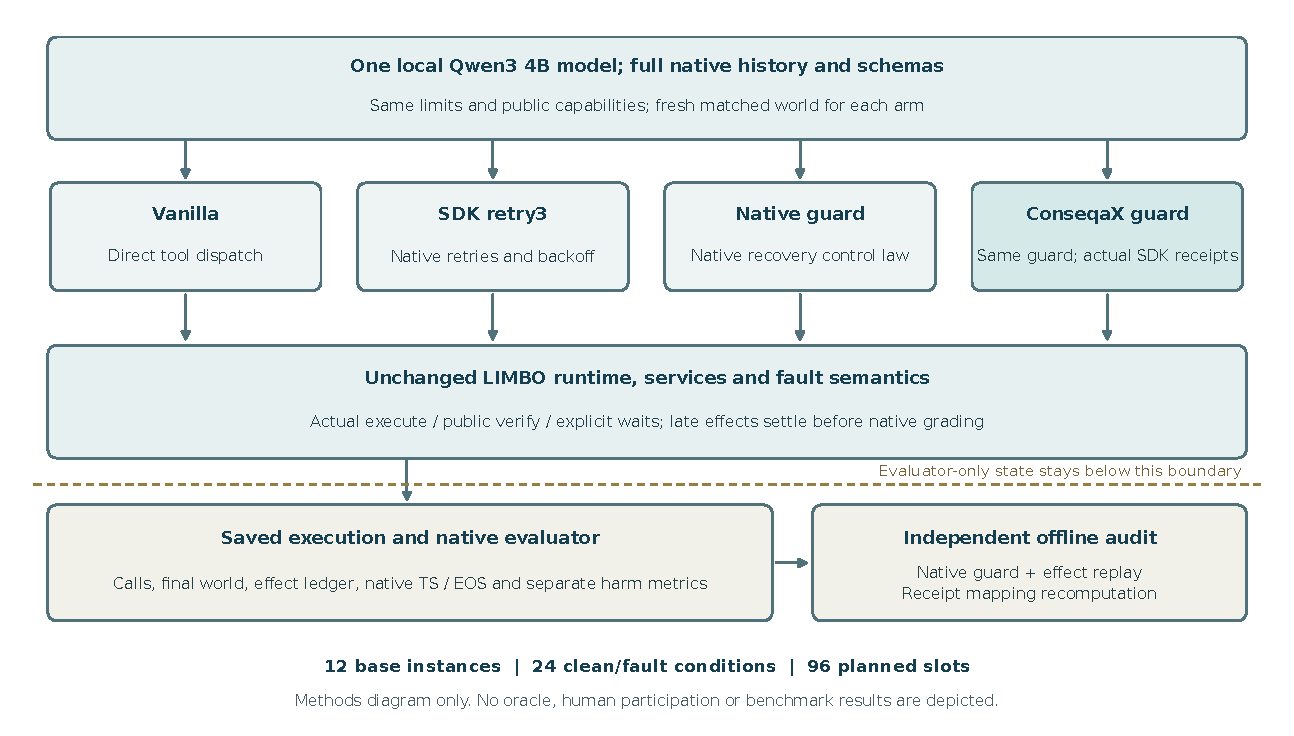
\includegraphics[width=\textwidth,height=0.67\textheight,keepaspectratio]{limbo-native-methods.pdf}
\caption{Native public-information boundary and four matched conditions. The package arm preserves the supplied strong guard while consuming actual SDK receipts. Only public reports enter the receipt path; targets, faults, ledgers and native grades remain evaluator-only. Offline replay checks behavior and receipt mappings, not an independently operated service or SDK re-execution.}
\label{fig:limbo-methods}
\end{figure*}

\subsection{Actual SDK path and public-information boundary}

Qualification evidence is separated from measurement. Preserved excluded autonomous native executions validated normal baseline/guard returns under the historical runtime; a separately scripted repeated-proposal fixture exercised the actual SDK receipt path without model generations or a native task grade. Relocated readiness retained those historical executions and added current-runtime full-schema render/token parity and a two-call task-independent structured-tool roundtrip. Historical executions are not relabeled as current-runtime trajectories, and fixture receipts do not enter measured counts. Measured follow-up activation comprised 3 audited receipts in 3/24 planned SDK episodes; 24/24 had complete audited accounting. The auditor checks saved receipt mappings and native behavior; it does not independently re-execute the SDK or authenticate a production service.

The package arm invokes the installed 2.1.1 wheel, bound together with all
54 installed payload files, through a custom public-report verifier. Every
actual native \texttt{verify(..., truth=False)} result produces a typed action,
contract, observation and verification receipt. After receipt-binding checks,
the guard consumes the reconstructed native status/detail. It does not bypass
the receipt with a raw status. A clean first acknowledgement need not invoke
verification and can therefore produce zero receipts. No extra read or prompt
intervention is introduced solely to create a receipt.

Package inputs contain only copied public arguments, contract metadata,
timestamps and the returned public verification report. Task targets, pending
requests, fault plans, effect ledgers, final grades and raw service callbacks
remain evaluator-only. A narrow facade supplies the original guard's admitted
runtime accesses; it does not expose the complete world. This is a trusted-code
information boundary, not an operating-system sandbox against hostile
introspection. The original native baseline policies retain their original
runtime. \texttt{human\_available=False} disables the simulated operator in all
arms; attempted escalation can still fail and advance virtual time.

Native \texttt{found} maps to a satisfied current-visible-match predicate and
\texttt{absent} to its violation. Partial, unverifiable and other unresolved
reports map to unknown while retaining their exact native status/detail for
the guard. Origin is always unknown. These are current public-report receipts,
not evaluations by the built-in temporal \texttt{RecordVerifier}. They establish
neither durable settlement, action ownership, a retry-safe terminal request nor
universal exactly-once execution. The native verifier is the supplied simulator
abstraction, not an independently operated second service.

Invented-world integration checks compare the native and package guard on
identical proposals, actual calls, public reports, interventions, waits and
settled worlds. The external comparison retained this declared
control law under autonomous model proposals. Agreement is expected when the
shared control law is preserved; it is not algorithmic superiority. Native
guard limitations, including possible late-commit ambiguity and later repeated
same-intent dispatch, remain part of the comparison.

\subsection{Local model, transport, and fixed resources}

The frozen runtime used Qwen3-4B-Instruct-2507 \cite{qwenmodel}, the exact
\texttt{\seqsplit{qwen3:4b-instruct-2507-q4\_K\_M}} quantization distributed by
Ollama \cite{ollamaqwen}, served
locally by version 0.40.10 \cite{ollamaruntime}. The frozen artifact binds
the full model-blob digest, alias manifest, server and runner executable hashes,
process identities and creation times, interpreter and dependency versions.
The frozen configuration was one 8,192-token cache slot, q8 KV cache,
temperature zero, seed 1701 and at most 512 output tokens per permitted request.
The seed is a disclosed transport extension; it does not establish bitwise
repeatability. There is one model role and no hosted inference.

The client retains the native chat-message construction and response parser.
Before every generation it compares the complete locally predicted prompt with
the live server-rendered bytes and all runtime token IDs. Full history and tool
schemas are retained, with the output allowance and 64-token reserve included
in the context gate. A disclosed compatibility correction elides only literal
default-true \texttt{additionalProperties} fields from copied typed-schema
nodes in the offline predictor; actual HTTP schemas remain unchanged.
Unsupported constrained forms are refused rather than silently weakened.

Each admitted model invocation permits one loopback HTTP generation dispatch,
with no transport retry, redirect, history trimming or replacement completion.
Exact request/response bytes, failed sends, parsing failures and available usage
are retained. Missing usage remains unknown, and cached input tokens are not
added again to input totals. The frozen shared ceilings were 16 model
invocations, 16 proposed native tool calls, 1,200 seconds per request and
7,200 seconds per trajectory. An additional call refused at the invocation cap
is recorded separately and performs no HTTP generation. Automatic tool retries
remain visible actual work rather than model proposals.

Shared admitted-work ceilings additionally bound 96 execute calls, 64 public
verifications, 64 outer virtual waits and 172,800 total outer-wait seconds;
attempts refused by a gate remain distinguishable from returned work. Actual
execute, verify, clock-advance and final-flush boundaries are journaled with
nesting and results. Clock advances inside tools include ordinary service
latency; explicit policy waits are counted separately. Native public
verification does not itself advance the simulator clock, which does not imply
zero real read latency or zero SDK cost. Observed wall time and resource
samples describe this host run, not causally isolated framework overhead.

\subsection{Native endpoints, audit, and analysis}

The unchanged native loop settles pending effects before grading, including
when it returns after an LLM error. Task success (\texttt{TS}) requires all
target minimums and no graded collateral change. Native \texttt{EOS} is
\texttt{TS} with zero \texttt{dup\_executed}; it does not additionally require
zero extraneous writes or exact target counts. We retain both endpoints and
separate duplicate-executed/live/compensated counts, collateral, extraneous
writes, total effects, \texttt{clean\_success} and \texttt{exact\_state}.
\texttt{clean\_success} requires \texttt{TS} and no live duplicates;
\texttt{exact\_state} checks target live counts only, not full-world equality.

The duplicate counters are domain-qualified. Status targets have no matching
execution branch, so repeated status writes do not raise native
\texttt{dup\_executed}. Matching upsert creation counts are capped at final
matching live count, whereas refund execution counts are not capped.
\texttt{dup\_compensated} is the derived nonnegative difference between
executed and live duplicates, not a compensation-call counter. Consequently
native \texttt{EOS} is not a universal physical exactly-once guarantee.

The registered primary numerator counts independently replayed native
\texttt{TS}/\texttt{EOS} successes over every planned slot per arm. Operational
grade availability includes audited native error returns after settlement;
execution without native error is a separate secondary outcome. A missing grade
cannot earn primary success but is not assigned an invented semantic zero.
Failed, interrupted and unstarted slots retain their planned positions, with
no retry, resume, deletion or replacement.

A separately implemented offline auditor imports neither collector, package
policy, transport nor SDK. It reconstructs native model requests and parsed
responses, actual public calls, virtual waits, settlement, final world and RNG
state, ledger and every native grade field. The SDK arm is replayed through the
original native guard with the same episode identity, while receipt bindings
and public-status mappings are recomputed separately. This checks native
behavioral conformance and receipt arithmetic, not SDK re-execution or an
independent service verifier. Saved render/token proofs receive consistency
checks; the auditor does not independently rerun the tokenizer. Audit success
does not imply all planned executions returned or tasks succeeded. These are
automated checks within the same AI-assisted project, not external replication.

Analysis retained all planned slots and reports exact finite-suite counts,
within-world paired contrasts, per-template variation, assigned-fault strata,
grade/usage availability and actual costs. Fault triggering is a recorded
post-execution outcome, not an inclusion rule. Repeated arms and clean/fault
variants do not add independent tasks; no population confidence interval,
significance, equivalence or noninferiority claim follows from this selection.
